% --------------------------------------------------------------- %
%%                                                               %%
%%%                                                             %%%
%%                                                               %%
% --------------------------------------------------------------- %
\section{Software Framework}
%

\begin{figure}
  \centering
  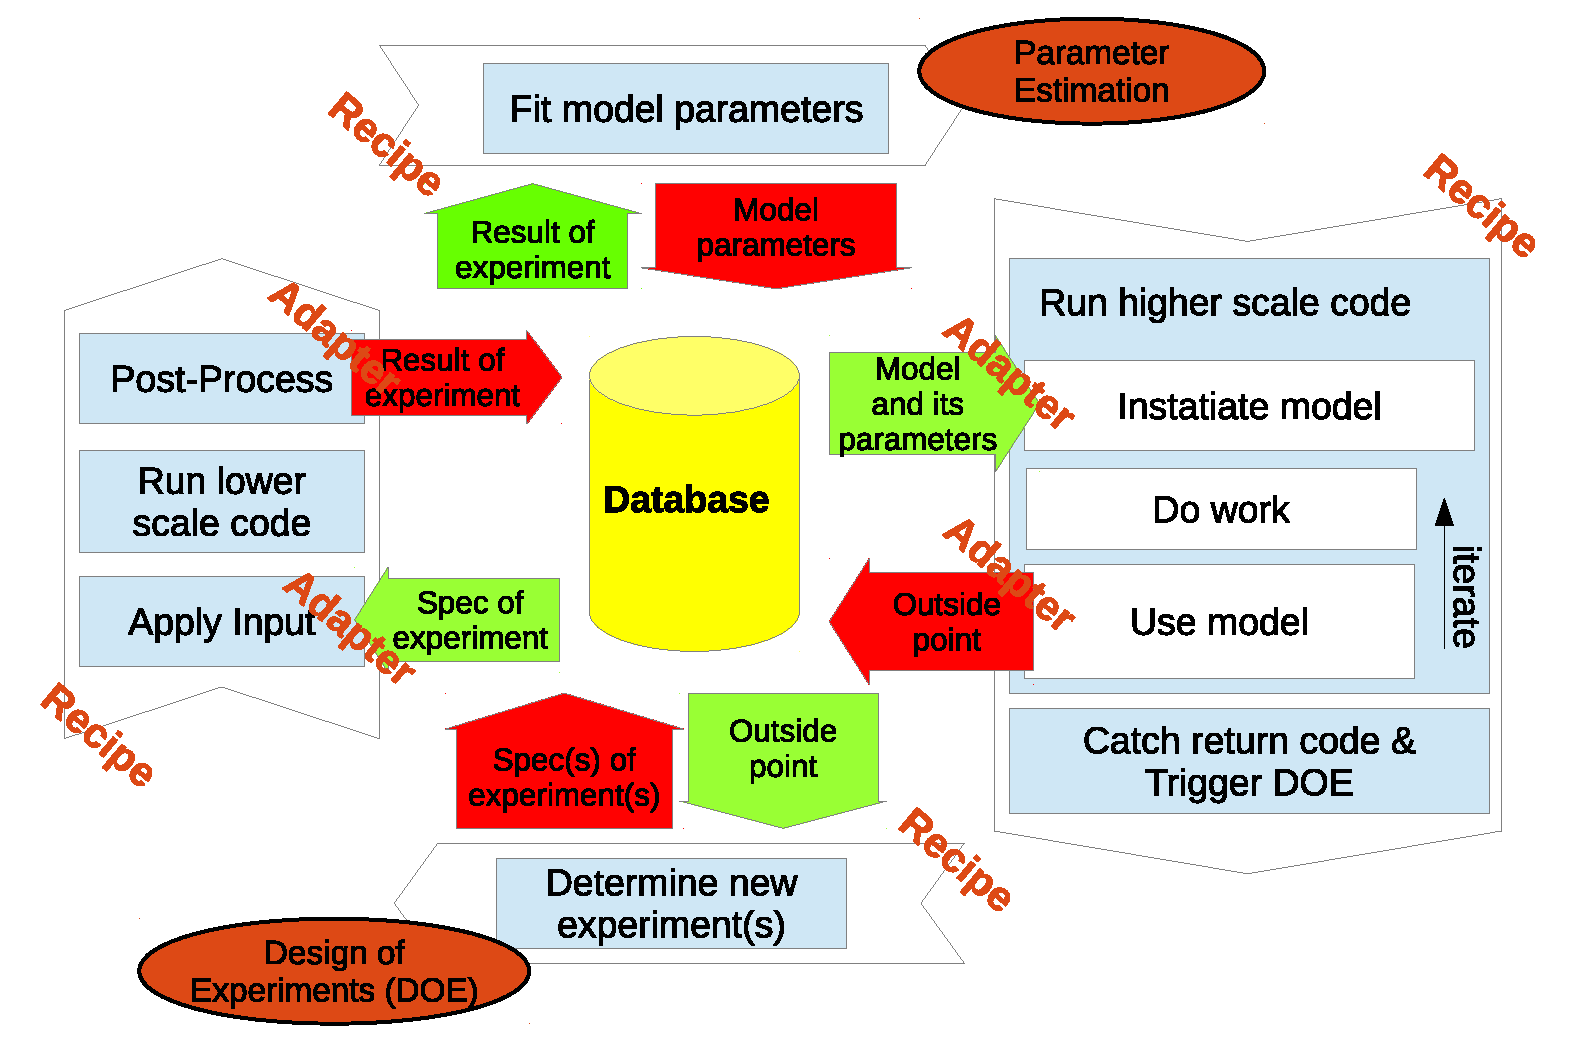
\includegraphics[width=0.75\textwidth,keepaspectratio=true]{./Content/Figures/Data_Flow.eps}
  \caption{The flow of data in the {\MoDeNa} concept.
  }
  \label{fig:DataFlow}
\end{figure}

The {\MoDeNa} software framework handles the communication across scales through
recipes and adapters ss shown in Figure \ref{fig:ConceptualStructure} and
\ref{fig:DataFlow} . Recipes perform simulations by executing applications
(in-house codes or external software packages such as FOAM, Materials Studio,
Predici) for a given set of inputs.  Adapters handle the communication with the
{\MoDeNa} software framework.  Both, recipes and adapters are application
specific.  Adapters exist as outgoing and incoming adapters.  Outgoing adapters
are relatively straight forward in that they perform a mapping operation (such
as averaging) and communicate the results. The averaging process may have to be
started and performed within the application (e.g.  for time averaging).
However, the results can usually be submitted in a separate process after the
simulation is finished. Incoming adapters are more complicated since they
usually require to embed surrogate models within the applications.

\begin{figure}
  \centering
  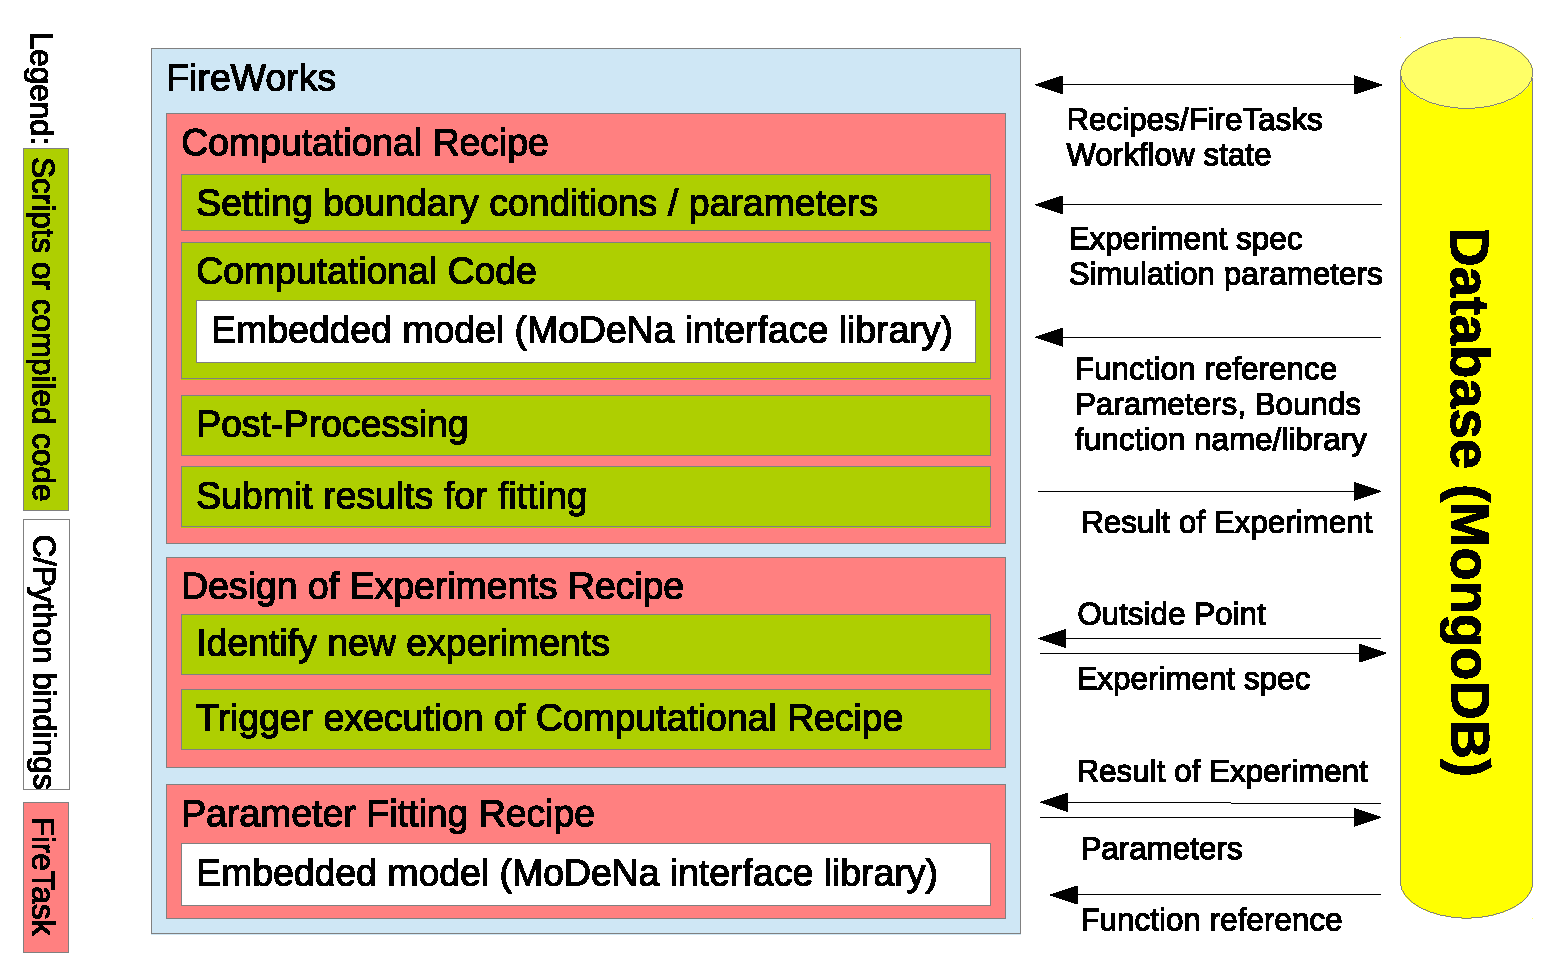
\includegraphics[width=0.75\textwidth,keepaspectratio=true]{./Content/Figures/Software_Stack.eps}
  \caption{The {\MoDeNa} software stack.
  }
  \label{fig:SoftwareStack}
\end{figure}

As shown in Figure \ref{fig:SoftwareStack}, the software framework consists of
an orchestrator, a database and a interface library. The orchestrator is based
on FireWorks \cite{project:FireWorks} and constitutes the backbone of the
software framework in that it schedules simulations as well as design of
experiments and parameter estimation operations which make up the work-flow of
the overall simulation. It is very much like a dynamic work-flow engine, in
which the different applications are ``orchestrated'' to obtain information,
analyse and pass it to the other operations. The {\NoSQL} database {\MongoDB}
\cite{project:MongoDB} is used to store the state of the work-flow as well as
the surrogate models together with associated data such as model parameters,
data used for parameter estimation, and meta-data.

The interface library consists of two parts: A high-level python module
providing access to the database as well as design of experiments and parameter
estimation capabilities by building on MongoEngine \cite{project:MongoEngine}
and R \cite{project:R}, respectively. The second part is a low-level library
providing unified access to the surrogate models. This component is written in C
to ensure interoperability across platforms and target applications while
providing the computationally efficient model execution required by the
applications.  The library is loaded as a shared library by the
macroscopic-scale applications or as a native python extension by the high-level
python module ensuring that all components instantiate identical model
implementations. Complex operations such as database access are referred back to
the high-level python module using call-back mechanisms.
